% experiments.tex

\cs{todo: discuss differences between domains}
\gbt{Not sure we'll have space :) }

We use \mn to gain insight into the extent to which current models account for object naming.
We do so in three ways: By analyzing the behavior of existing models on entry-level names, by assessing the consequences of fine-tuning models with entry-level name data, and by analyzing the predictions of the models, comparing them to human naming behavior as attested in \mn.
The latter will be done in Section~\ref{sec:analysis}; here we focus on modeling experiments.
\gbt{Maybe this needs to go in the intro or somewhere else. It's important to stress that the modeling experiments are on entry-level only, and the analysis takes into account the other names.}

The modeling experiments adopt the standard single-label object classification approach of Computer Vision, and we will compare prediction of the original \vg name with the entry-level name.
We leave modeling experiments that take into account other possible names of objects for future work.

% Our goal is to experimentally obtain insights into the usefulness of computer vision object labeling models, that are commonly used for \lv methods, to account for natural human object naming. 
% Specifically, our research questions are
% \begin{enumerate}
% 	\item Do object detection models, despite being trained on \arbitrary  
% 	names, account for human object naming?\cs{repetitive}
% 	\item Can we apply simple transfer learning on \mn to train classifiers towards this naming task by utilizing pre-trained object detection or image classification model as feature extractors? Figure~\ref{fig:exp_confusions} \\
% 	\cs{move to models: -- can we learn entry-level names by fine-tuning object detection models on \mn?\\
% 		-- Can we directly learn entry-level names by fine-tuning image classification models on \mn, i.e.,\ the pre-trained features to initialize object detection models?}
% \end{enumerate}
% TO BE COVERED BY THE SUBSECTIONS BELOW:
% \begin{enumerate}
% 	\item Do models prefer the entry-level name of an object over an \arbitrary name? Table~\ref{tab:exp_VGvsMN}
% 	\item In cases of failure, do they predict alternative, but less preferred  names instead? Tables~\ref{tab:exp_overview_results}, \ref{tab:exp_alternatives}
% 	\item What phenomena of human behavior on the object naming task of \mn do the models mirror? That is, which model mistakes or confusions are due to the artificial setup of the task itself, and less a failure of the model? (Recall that \mn serves as a \textit{proxy} for natural human object naming, since annotators were asked to name a highlighted object in an image isolated from its situative context; Section~\ref{sec:manynames}) Table~\ref{tab:exp_details_wrong} (and \ref{tab:exp_errors_agreement},  \ref{tab:exp_alternatives})
% \item \cs{Not examined at the moment -- MRR and Jaccard may be re-added for this: Are valid name alternatives among the top-N predictions?}
%\item do we get different evaluation results when testing existing object classification models on preferred responses from name distributions, as compared to naming responses collected from 1-3 workers (e.g., VisualGenome)? 
%\end{enumerate}

\subsection{Experimental Setup}
\label{sect:exp_setup}

\paragraph{Data}
\gbt{I moved this here cause I think it will be useful to define the different vocabularies here and then be able to simply refer to them later. Btw, consider using `MN-Entry' instead of `MN442'? but maybe having the number in the name is useful to be able to compare.}
\cs{todo after Section~\ref{sect:mn_overview} has been written.}
\begin{itemize}
	\item Test data: overlap of \mn and \vg test data (CITE)
	\item Target vocabulary of test data: overlap of MN442 and VG (\cs{XX} names)
	\item Source of label: \mn, but we compare against \vg
\end{itemize}

\paragraph{Models}

We test 1) an existing object detection and classification model trained on \vg (FRCNN$_{\text{VG1600}}$); 2) the same model, re-trained on the smaller vocabulary of entry-level names, MN442 (FRCNN$_{\text{MN442}}$); 3) an object classification model trained on FRCNN$_{\text{VG1600}}$ features, that is, a version of FRCNN$_{\text{VG1600}}$ fine-tuned on \mn data (FRCNN$_{\text{VG1600}}$$_{\text{-VGMN}}$ \gbt{find better name?}); 4) object classification models trained directly on object detection features (given by ResNet 101; \cite{}), rather than object classification features.

FRCNN$_{\text{VG1600}}$ is the bottom-up attention model of \citeauthor{anderson2018updown}'s \citeyear{anderson2018updown},\footnote{Available at \url{https://github.com/peteanderson80/bottom-up-attention}. The model is trained with an additional output over attributes, but we only use the object class prediction layer.}
trained to do object classification with a vocabulary of $1600$ VG names as class labels. \cs{add how the vocabulary was derived}.
The model is based on the object detection \gbt{detection, or classification?} method Faster R-CNN \cite{fasterrcnn2015}. 
The authors initialized it with ResNet-101 \cite{he2016deep} features (pretrained on ImageNet) to then train it on \vg.
To train FRCNN$_{\text{MN442}}$, we follow the same methodology as in \citeauthor{anderson2018updown} \cs{right, @Sina?} but restrict the object classes to the $442$~entry-level names found in \mn; accordingly, we train on fewer images. \gbt{Right? Only those that have an entry-level name? TODO: add how many imgs for FRCNN$_{\text{VG1600}}$ and FRCNN$_{\text{MN442}}$.}
\gbt{Also, Do we also use the additional attribute loss?}
\footnote{For training, we use a PyTorch reimplementation of Faster R-CNN, \url{github.com/jwyang/faster-rcnn.pytorch}.}
FRCNN$_{\text{MN442}}$ serves us to test the hypothesis that training only on entry-level names may improve generalization and hence performance.

The two former models are trained on \vg, which has almost 4 million labeled objects.
\mn is too small to train object detection models on it from scratch, which require learning millions of parameters.
On the other hand, obtaining enough naming data to be able to estimate entry-level names for larger datasets is very costly --probably unrealistic.
Therefore, we investigate the possibility of obtaining entry-level data via transfer learning, fine-tuning existing models with \mn data.
We do so with the standard methodology \gbt{in L\&V?} of taking the last hidden layer of existing Computer Vision models as input, and train object classification models to predict entry-level names (MN442).

We experiment with two kinds of input. First, the features from the object classification model FRCNN$_{\text{VG1600}}$\footnote{As our experimental results will show, FRCNN$_{\text{VG1600}}$ is more effective than FRCNN$_{\text{MN442}}$, so we only use the former model.}. 
We expect these to be very good features for our task, as they have been obtained with the same task (object classification) and dataset (\vg).
For comparison, we consider a much less informed kind of input, namely the features from an object detection model, ResNet-101 \cite{+++}, which are the ones that FRCNN$_{\text{VG1600}}$ use as initialization features. \gbt{Previous sentence to be improved}
Results should of course be worse, and our aim is to assess the feasibility of using such generic object representations to obtain entry-level names.

\cs{Next sentence relevant here? Or just as detail in related work?:: (Note that ResNet's $1$K~object classes capture subordinate categories of ImageNet leaf nodes; e.g.,~Siberian husky, American black bear.)} 

\gbt{begin not integrated}
As with the FRCNN models above, we compare models which differ in  their target vocabulary, i.e.,~VGMN or MN442. 
\cs{Maybe the next sentences are better just in the results section, when discussing the table::} Finally, we compare against two further classifiers which are trained on the \vg labels. 
Note that all four models are optimized on the $25$K~objects in \mn. 
\gbt{end not integrated}

\gbt{IMPORTANT: I would not include all four ResNet models in the main paper; it takes a lot of space in all the result tables and also the explanation and doesn't add much information. I'd put the most relevant (at most two, maybe even only one) in the main paper and leave the rest for the supplementary material. TBD}

\cs{todo: details to architecture and training of the vanilla classifiers.}
\gbt{I leave this here unchanged:} For each object (i.e.,~bounding box) in \mn, we extract its activation features from FRCNN's last hidden layer before the output layer.\cs{add size} 
To predict the entry-level name of a target object~$o$, the classifier, a multi-layer neural network, is fed the object's features, and applies softmax activation to the output layer that corresponds to the target vocabulary. 
The target vocabulary (VGMN, henceforth) comprises the overlap of VG1600 and the \mn names (\cs{$XX$} in total). \gbt{All \mn names? or only MN422? To be clarified above under paragraph `Data'.}

\begin{table}[t]
	\centering
	\small
	\begin{tabular}{@{~}l@{~}|@{~}c@{~}|cc|cc@{~}}
		\toprule
		&  & \multicolumn{2}{c}{All} 
		& \multicolumn{2}{c}{VG$\neq$MN}\\
		&  & \multicolumn{2}{c}{($1072$)} 
		& \multicolumn{2}{c}{($223$)}\\	
		Model$_{\text{Vocab}}$ 
		&  GTtrain &  VG & MN 
		&  VG & MN \\ 
		\midrule
		FRCNN$_{\text{MN442}}$ & VG &  65.4 &      71.2 &   20.0 &      48.4  \\
		FRCNN$_{\text{VG1600}}$ & VG &    67.3 &      74.5 &    19.1 &      52.9  \\
		\midrule \midrule
		\multicolumn{6}{c}{Classifiers: Transfer learning on MN}\\
		Features$_{\text{Vocab}}$ &   \\
		\midrule 
		FRCNN$_{\text{VG1600}}$$_{\text{-VGMN}}$ & MN &    70.8 &      80.6 &    13.8 &      60.4  \\ 
		\midrule
		ResNet$_{\text{VGMN}}$ & MN  & 60.9 &  68.6 &  13.8 & 50.2  \\
		
		ResNet$_{\text{MN442}}$ & MN &            61.7 &              69.6 &                        13.8 &              50.7 \\
		ResNet$_{\text{VGMN}}$  &   VG &  62.4 &              62.9 &              28.4 &              31.1  \\
		%ResNet$_{\text{VGMN}}$\_4ep  &   VG &  62.4 &              62.9 &              28.4 &              31.1  \\
		%ResNet101$_{\text{VGMN}}$\_8ep & VG &            63.9 &              62.6 &          34.2 &              28.0 \\
		ResNet$_{\text{MN442}}$ & VG  &            63.7 &              63.7 &                  30.7 &              31.1  \\
		\bottomrule
	\end{tabular}
	\caption{Model accuracy (in \%) on the \mn test objects. Vocab denotes the dataset used to induce the target vocabulary for training (the numbers give the size of the vocabulary). GTtrain gives the dataset that provides the ground truth labels during training, and VG and MN for testing \label{tab:exp_VGvsMN}.}
\end{table}


%\paragraph{Measures}


\subsection{Results: Entry-Level Name Prediction}
\label{sect:exp_results}
%\paragraph{Entry-Level Name Prediction}
Table \ref{tab:exp_VGvsMN} shows the accuracy of all models on the \mn test data. 
We compare model effectiveness on predicting the entry-level name (columns MN) against predicting the \arbitrary VG name (columns VG), and furthermore report results on the test instances where the two names differ (block VG$\neq$MN). 
\begin{itemize}
	\item The FRCNN models are better on predicting the entry-level name (columns MN) than the \arbitrary VG name (columns VG). 
	This shows that they do learn entry-level naming to some extent, despite being trained on VG, i.e.,~\arbitrary ground truth labels.
	\cs{I would not comment on diff. btw. the two FRCNNs, it's small compared to their diffs to the classifiers, and may be also due to the diff. implementations, and VG1600 being trained additionally on attributes.}
	\item The overall best model is FRCNN$_\text{VG1600}$$_\text{-VGMN}$, the Vanilla classifier that uses  FRCNN$_\text{VG1600}$ features and is trained on the \mn training data. 
	\item \cs{?What to keep here:} The classifiers using ResNet features are the least effective, but come close to the FRCNN object detectors on entry-level naming (columns MN, GTtrain MN), or even better  (columns VG, GTtrain VG) despite being trained on a fraction of FRCNN's training size using a simple Vanilla classifier in contrast to a fully-fledged CNN architecture.
	This confirms what we observed on the FRCNN results: and follow the pattern of learning entry-level naming  
	\item Models learn entry-level naming when being trained on \arbitrary naming data, obtaining better results on entry-level prediction than \arbitrary name prediction for the same instances, and benefit from being trained on entry-levels using transfer learning. \cs{overfitting?}
	\item Comparing the target vocabulary, MN442 and VG1600/VGMN, we see that the restriction on a smaller, but empirically derived vocabulary of entry-level names only, is not beneficial, with all MN442 models being worse or comparable to VGMN/VG100.
\end{itemize}

\subsection{Quantitative Analysis}
\label{sect:exp_analysis}


\paragraph{Alternative Name Prediction}
\begin{figure}
	\centering
	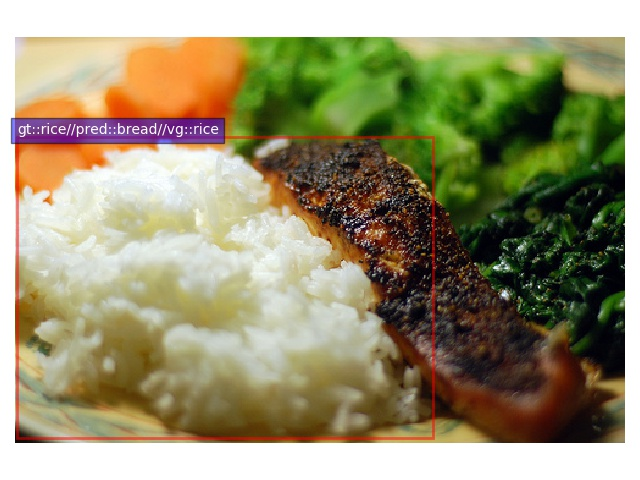
\includegraphics[scale=.2]{images/2323938.jpg}
	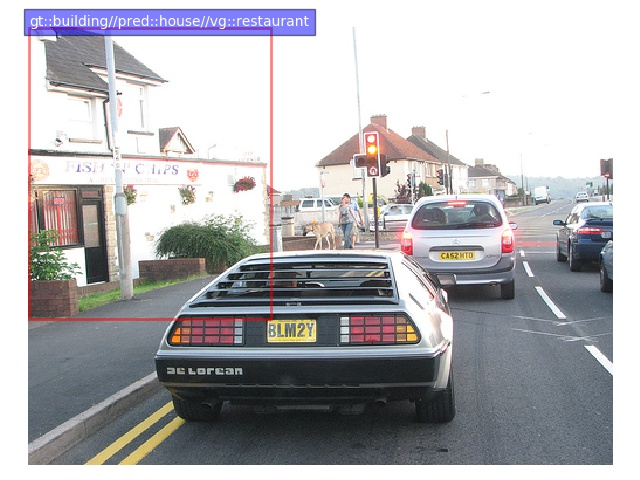
\includegraphics[scale=.2]{images/2322259.jpg}
	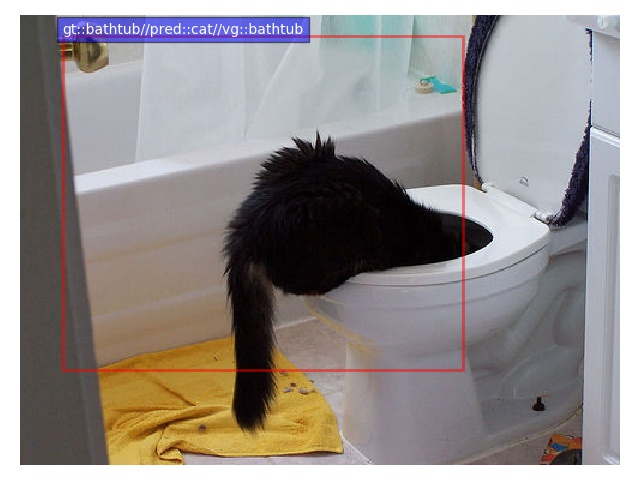
\includegraphics[scale=.2]{images/2371657.jpg}
	
	\caption{TODO: examples resnet mistakes (trained on vg\_manynames, tested on manynames-442)\label{fig:mistakes}}
\end{figure}

\cs{TODO::}
Categorization of "errors" (see Figure~\ref{fig:mistakes}):
\begin{enumerate}
	\item Clear mistake \\
	e.g.,\ rice vs. bread
	\item Alternative name\\
	e.g.,\ building vs. house
	\item Alternative object \cs{(other cluster from verif data)}
	\item Synonym\\
	e.g.,\ plane vs. airplane
	\item Semantically related\\
	e.g.,\  motorcycle vs. scooter
\end{enumerate}

\begin{table*}[t]
	\centering
	\small
	\begin{tabular}{l|c|r@{~}r@{~}r@{~}||r@{~}r@{~}r@{~}}
		\toprule
		& & \multicolumn{3}{c}{All Test Images ($\#$)} 
		& \multicolumn{3}{c}{VG$\neq$MN Images ($\#$)}\\
		\toprule
		Model$_{\text{Vocab}}$	& GTtrain  
		&  hit &  correct &  incorrect &  hit &  correct &  wrong \\
		\midrule
		FRCNN$_{\text{VG1600}}$ & VG           &         74.8 &                  13.9 &                    11.3 &         54.3 &                  30.0 &                    15.7 \\
		FRCNN$_{\text{MN442}}$ & VG &         71.1 &                  13.9 &                    15.0 &         48.4 &                  28.7 &                    22.9 \\
		\midrule \midrule
		FRCNN$_{\text{VG1600}}$$_{\text{-VGMN}}$ & MN %&         0.81 &                  0.09 &                    0.11 &         0.60 &                  0.23 &                    0.17 \\
		&         80.7 &                   9.2 &                    10.1 &         60.1 &                  23.8 &                    16.1 \\
		\midrule
		ResNet101$_{\text{MN442}}$ & MN %& 0.70 &                  0.09 &                    0.21 &         0.51 &                  0.22 &                    0.27 \\
		&         69.7 &                  10.3 &                    20.1 &         51.1 &                  23.3 &                    25.6 \\
		ResNet101$_{\text{VGMN}}$ & MN% &         0.69 &                  0.09 &                    0.22 &         0.51 &                  0.23 &                    0.26 \\	
		&         68.7 &                  10.5 &                    20.8 &         50.7 &                  24.2 &                    25.1 \\
		ResNet101$_{\text{VGMN}}$ & VG %&         0.63 &                  0.11 &                    0.26 &         0.31 &                  0.28 &                    0.40 \\
		&         62.8 &                  12.6 &                    24.6 &         31.4 &                  30.0 &                    38.6 \\
		ResNet101$_{\text{MN442}}$ & VG %&         0.64 &                  0.11 &                    0.25 &         0.32 &                  0.29 &                    0.39 \\
		&         63.8 &                  12.6 &                    23.6 &         32.3 &                  30.0 &                    37.7 \\
		\bottomrule
	\end{tabular}
	\caption{Break-down of the results (in \%): Categorization of a predicted name\ $\hat{n}$ into either a \textit{hit} (exact match with entry-level name, cf. standard evaluation), \textit{correct} (less preferred name, synonym, hypernym/hyponym), or \textit{wrong} (wrong object, $\text{count}(\hat{n})<2$, co-hyponym, clear mistake). \label{tab:exp_overview_results}}
\end{table*}

\begin{table*}[t]
	\centering
	\small
	\begin{tabular}{l|c|rrr||rrr}
		\toprule
		& &  \multicolumn{3}{c||}{MN agreement $>$ 0.9} & \multicolumn{3}{c}{MN agreement $\leq$ 0.9}\\
		Model$_{\text{Vocab}}$ &  GTtrain & hit &  correct &  incorrect &  hit &  correct &  incorrect \\
		\midrule
		FRCNN$_{\text{VG1600}}$ & VG &      94.8 &           1.8 &             3.4 &     63.6 &         24.5 &           12.0 \\
		FRCNN$_{\text{MN442}}$ & VG &      89.6 &           1.6 &             8.8 &     60.7 &         23.9 &           15.4 \\
		\midrule \midrule
		FRCNN$_{\text{VG1600}}$$_{\text{VGMN}}$ & MN &      94.5 &           1.3 &             4.2 &     72.9 &         16.5 &           10.6 \\
		\midrule 
		ResNet101$_{\text{VGMN}}$ & VG &      88.3 &           1.8 &             9.9 &     48.5 &         23.6 &           27.8 \\
		ResNet101$_{\text{VGMN}}$ & MN &      89.6 &           1.6 &             8.8 &     57.0 &         19.4 &           23.6 \\
		ResNet101$_{\text{MN442}}$ & MN &      90.1 &           1.3 &             8.6 &     58.2 &         19.5 &           22.3 \\
		\bottomrule
		
	\end{tabular}
	\caption{Break-down of the results (in \%) according to the agreement level of the MN name: Categorization of a predicted name\ $\hat{n}$ into either a \textit{hit}, \textit{correct} (less preferred name, synonym, hypernym/hyponym), or \textit{wrong} \label{tab:exp_errors_agreement}}
\end{table*}

\begin{table*}[t]
	\centering
	\small
	\begin{tabular}{l|c|r@{~}|r@{~}r@{~}r@{~}r@{~}r@{~}||r@{~}|r@{~}r@{~}r@{~}r@{~}r@{~}}
		\toprule
		& & \multicolumn{6}{c}{All Test Images ($\#$)} 
		& \multicolumn{6}{c}{VG$\neq$MN Images ($\#$)}\\
		\toprule
		Model$_{\text{Vocab}}$ &  GTtrain & same &  syn. &  syn. &  hyper. &  hypo. &  hyper. &  same &  syn. &  syn. &  hyper. &  hypo. &  hyper. \\
		& 	&  cluster &  & cluster & & & cluster 
		& cluster  &  & cluster & & & cluster \\
		\midrule
		FRCNN$_{\text{VG1600}}$ & VG     %        &                  0.95 &              0.0 &                0.01 &              0.01 &             0.03 &                 0.0 &                  0.96 &              0.0 &                 0.0 &              0.01 &             0.03 &                 0.0 \\
		&                  94.6 &              0.0 &                 0.7 &               3.4 &              1.3 &                  0.0 &                  95.5 &              0.0 &                 0.0 &               3.0 &              1.5 &                  0.0 \\
		FRCNN$_{\text{MN442}}$ & VG %&                   0.97 &             0.01 &                0.02 &               0.0 &              0.0 &                 0.0 &                  0.97 &              0.0 &                0.03 &               0.0 &              0.0 &                 0.0 \\
		&                  93.3 &              1.3 &                 2.0 &               1.3 &              2.0 &                  0.0 &                  93.8 &              0.0 &                 3.1 &               1.6 &              1.6 &                  0.0 \\
		\midrule \midrule
		FRCNN$_{\text{VG1600}}$$_{\text{VGMN}}$ & MN %&                   1.0 &              0.0 &                 0.0 &               0.0 &              0.0 &                 0.0 &                   1.0 &              0.0 &                 0.0 &               0.0 &              0.0 &                 0.0 \\
		&                  94.9 &              0.0 &                 0.0 &               2.0 &              3.0 &                  0.0 &                  96.2 &              0.0 &                 0.0 &               1.9 &              1.9 &                  0.0 \\
		\midrule
		ResNet101$_{\text{VGMN}}$ & MN %&                  0.97 &              0.0 &                0.03 &               0.0 &              0.0 &                 0.0 &                  0.98 &              0.0 &                0.02 &               0.0 &              0.0 &                 0.0 \\
		&                  83.9 &              0.0 &                 2.7 &               6.2 &              5.4 &                  1.8 &                  92.6 &              0.0 &                 1.9 &               1.9 &              3.7 &                  0.0 \\
		ResNet101$_{\text{MN442}}$ & MN %& 0.97 &              0.0 &                0.03 &               0.0 &              0.0 &                 0.0 &                  0.98 &              0.0 &                0.02 &               0.0 &              0.0 &                 0.0 \\
		&                  86.4 &              0.0 &                 2.7 &               5.5 &              3.6 &                  1.8 &                  92.3 &              0.0 &                 1.9 &               1.9 &              3.8 &                  0.0 \\
		ResNet101$_{\text{VGMN}}$ & VG %&                   0.98 &              0.0 &                0.02 &               0.0 &              0.0 &                 0.0 &                  0.98 &              0.0 &                0.02 &               0.0 &              0.0 &                 0.0 \\
		&                  87.4 &              0.0 &                 2.2 &               1.5 &              8.1 &                  0.7 &                  92.5 &              0.0 &                 1.5 &               1.5 &              4.5 &                  0.0 \\
		ResNet101$_{\text{MN442}}$ & VG% &                  0.98 &              0.0 &                0.02 &               0.0 &              0.0 &                 0.0 &                  0.97 &              0.0 &                0.03 &               0.0 &              0.0 &                 0.0 \\		
		&                  88.9 &              0.0 &                 2.2 &               2.2 &              5.9 &                  0.7 &                  92.5 &              0.0 &                 3.0 &               1.5 &              3.0 &                  0.0 \\
		\bottomrule
	\end{tabular}
	
	\caption{Break-down of the results for the \textit{correct} name predictions. Proportions (in \%) of the \textit{correct} categories to all correctly classified instances.  \textit{hyponym}: $\hat{n}$ is a hyponym of the entry-level name. \textit{hypernym\_cl}: $\hat{n}$ is a hypernym of any of the valid names (cluster). \textit{Synonym} and \textit{synonym\_cl} are analogous. \label{tab:exp_alternatives}}
\end{table*}

\paragraph{Incorrect Predictions}

\begin{table*}[t]
	\centering
	\small
	\begin{tabular}{l|c|r@{~}|r@{~}r@{~}r@{~}r@{~}|r@{~}r@{~}||r@{~}|r@{~}r@{~}r@{~}r@{~}|r@{~}r@{~}}
		\toprule
		&& \multicolumn{7}{c}{All Test Images ($\#$)} 
		& \multicolumn{7}{c}{VG$\neq$MN Images ($\#$)}\\
		\toprule
		Model$_{\text{Vocab}}$ & GTtrain  
		&  co- &  \multicolumn{4}{c}{other object}  &  error &  low 
		&  co- &  \multicolumn{4}{c}{other object}  &  error &  low \\
		& & hypo. & (vis. &  ling. &  box &  other)   & & count 
		&  hypo. & (vis. &  ling. &  box &  other) &   & count     \\
		
		\midrule
		FRCNN$_{\text{VG1600}}$ & VG     &                 13.2 &             1.7 &                 0.0 &                  17.4 &            6.6 &           39.7 &             21.5 &                  5.7 &             5.7 &                 0.0 &                  17.1 &           14.3 &           42.9 &             14.3 \\
		FRCNN$_{\text{MN442}}$ & VG       &                 15.5 &             0.6 &                 0.0 &                  15.5 &            6.2 &           49.1 &             13.0 &                  5.9 &             2.0 &                 0.0 &                  13.7 &           11.8 &           54.9 &             11.8 \\
		\midrule \midrule
		FRCNN$_{\text{VG1600}}$$_{\text{VGMN}}$ & MN &                 30.6 &             0.9 &                 0.0 &                  13.0 &            5.6 &           32.4 &             17.6 &                 16.7 &             2.8 &                 0.0 &                  16.7 &           11.1 &           41.7 &             11.1 \\
		\midrule
		ResNet101$_{\text{VGMN}}$ & MN	&                 34.1 &             0.0 &                 0.0 &                  13.0 &            1.3 &           39.5 &             12.1 &                 19.6 &             0.0 &                 0.0 &                  12.5 &            5.4 &           51.8 &             10.7 \\
		ResNet101$_{\text{MN442}}$ & MN  &                 33.0 &             0.0 &                 0.0 &                  14.0 &            1.9 &           37.7 &             13.5 &                 21.1 &             0.0 &                 0.0 &                  15.8 &            7.0 &           43.9 &             12.3 \\
		ResNet101$_{\text{VGMN}}$ & VG  &                 37.6 &             0.0 &                 0.0 &                   6.1 &            2.3 &           41.1 &             12.9 &                 24.4 &             0.0 &                 0.0 &                   3.5 &            5.8 &           45.3 &             20.9 \\
		ResNet101$_{\text{MN442}}$ & VG &                 34.0 &             0.0 &                 0.0 &                   7.5 &            2.8 &           41.9 &             13.8 &                 22.6 &             0.0 &                 0.0 &                   6.0 &            8.3 &           39.3 &             23.8 \\
		\bottomrule
	\end{tabular}
	\caption{Break-down of the results for the \textit{wrong} name predictions. Proportions (in \%) of the corresponding categories to all wrongly classified instances.  \label{tab:exp_details_wrong}}
\end{table*}

\paragraph{Human Object Naming through Transfer-Learning} Figure \ref{fig:exp_confusions} visualizes the change in predictions for  some of our retrained and finetuned models with respect to the object detection baseline (bottom-up-1600). For each object, where the new model predicts a different name than the baseline model, we look at the hit-error categories of the original and new predicted name. Observations:
\begin{itemize}
	\item Retraining faster-rcnn on less names does not lead to better calibration of entry-level names: more original hits change to same-cluster predictions than the other way round. (top left matrix)
	\item Finetuning the original faster-rcnn on many names recalibrates many decision from same-cluster names to the correct hit. Interestingly, also clear errors are calibrated to perfect hits, whereas hardly any error is changed to same-cluster or related.  (top right matrix)
	\item A similar tendency can be found for the ResNet models: finetuning ResNet on MN changes many predictions from same-cluster to hits. This is less the case when ResNet is finetuned on VG annotations.
	\item Interestingly, both ResNet models change hits into related names (hypernyms, hyponyms, cp-hyponyms) -- why does this happen?
\end{itemize}

\begin{figure*}[t]
	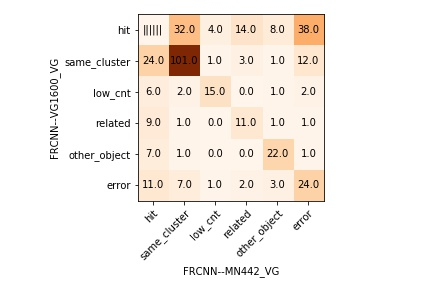
\includegraphics[scale=.5]{images/matrix_FRCNN--VG1600_VG_FRCNN--MN442_VG.jpg}
	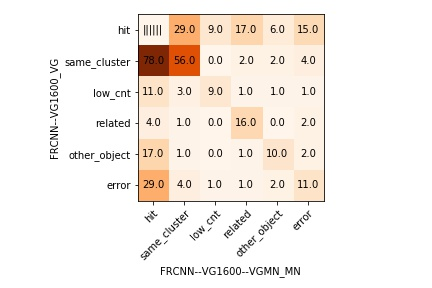
\includegraphics[scale=.5]{images/matrix_FRCNN--VG1600_VG_FRCNN--VG1600--VGMN_MN.jpg}
	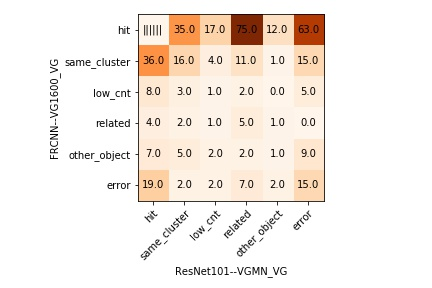
\includegraphics[scale=.5]{images/matrix_FRCNN--VG1600_VG_ResNet101--VGMN_VG.jpg}
	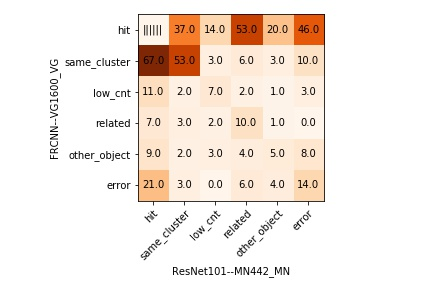
\includegraphics[scale=.5]{images/matrix_FRCNN--VG1600_VG_ResNet101--MN442_MN.jpg}
	
	\caption{Confusion-matrix-style visualization showing error categories of predictions that changed from object detection with FRCNN-VG1600 to naming with FRCNN-VG1600-VGMN (finetuned) \label{fig:exp_confusions}}
\end{figure*}


\subsection{Discussion}
\label{sect:exp_discussion}

%\iffalse
\cs{under construction}
\begin{itemize}
	\item Object detection models in CV have different goal than L+V object recognition models (see related work--former is on labels, latter on predicting natural language). 
	However, the former, pre-trained towards labels, are the backbone / used as feature extractors for the latter.
	\item ... 
	\item As we explained, there is a high variation of object names, and objects may be named by multiple alternative names (\cs{vocab size MN vs. vocab size VG for same object set}). 
	Yet, humans usually have a clearly preferred name for individual object instances (and the set of those is relatively small)--humans agree on a particular name for an instance (entry-level name).
	\item Hence, to model human object naming, datasets with many/dozens of annotations for the same instance are required. 
	\item We argue that such datasets are more reliable in that they provide empirically derived preferred names (entry-level names), and richer--the provide valid name alternatives. 
	\item But since their elicitation is expensive and time-consuming, it is not realistic to create training datasets of dozens of object names for pre-training features with CV models, which need a huge amount of training data. 
\end{itemize}
%\fi

\iffalse
We propose to use datasets of object names for evaluating models on the task of object naming (depending on results: also valuable for comparing object detection/image classification models).
Specifically, we analyse object detection [and classification] models on the task of human object naming, using the \mn dataset as test data:\\
Can object detection models, trained on arbitrary names, account for human object naming?
\begin{itemize}
	\item Do they predict the entry-level name?
	\item Are valid name alternatives among the top-N predictions?
	\item Do models make similar mistakes as humans when being faced with the task of naming highlighted objects in images [i.e.,\ the artificial setup of object naming for data annotation]?\\
	-- naming an alternative object (maybe more salient)\\
	-- predicting a semantically related name
	%do we get different evaluation results when testing existing object classification models on preferred responses from name distributions, as compared to naming responses collected from 1-3 workers (e.g., VisualGenome)? 
	\item Can we use \mn as fine-tuning dataset? (Here: only Vanilla model)\\
	-- can we learn entry-level names by fine-tuning object detection models on \mn?\\
	-- Can we directly learn entry-level names by fine-tuning image classification models on \mn, i.e.,\ the pre-trained features to initialize object detection models?
\end{itemize}
\fi

\iffalse
\subsection{[TBC] Predicting Entry-Level Names}
\label{sect:exp_entry}
Question: Can object detection models trained on a set of "arbitrarily" chosen object names account for entry-level object names? 

Note that the source dataset for defining the vocabulary (\textsl{Vocab}, i.e.,\ the overall set of considered names, i.e., the softmax layer's dimensions), and the source dataset which provides the ground truth names for the individual objects (\textsl{GTtrain}) may differ.  
\begin{table*}[t]
	\centering
	\small
	\begin{tabular}{l|c|r@{~}r@{~}r@{~}r@{~}r@{~}r@{~}r|@{~}r@{~}r@{~}r@{~}r@{~}r@{~}r@{~}r@{~}}
		\toprule
		&   & \multicolumn{6}{c}{All Test Images ($\#$)} 
		& \multicolumn{6}{c}{VG$\neq$MN Images ($\#$)}\\	
		Model$_{\text{Vocab}}$	 
		&  GTtrain &  =VG & =MN & $\in$MN  & KL & J & MRR & AvgMRR 
		&  =VG & =MN & $\in$MN  & KL & J & MRR & AvgMRR\\ 
		\midrule
		FRCNN--MN442 & VG &            65.4 &              71.2 &                85.6 &         1.0 &             69.8 &          0.8 &             0.7 &            20.0 &              48.4 &                78.7 &         1.4 &             60.4 &          0.7 &             0.5 \\
		FRCNN--VG2500 & VG \\
		FRCNN$_{\text{VG1600}}$ & VG &            67.3 &              74.5 &                89.2 &         0.6 &             74.3 &          0.8 &             0.7 &            19.1 &              52.9 &                86.2 &         0.8 &             69.4 &          0.7 &             0.6 \\
		\midrule \midrule
		& \multicolumn{12}{c}{Classifiers: Fine-tuning pre-trained image features on \mn}\\
		Features$_{\text{Vocab}}$ & GTtrain  \\
		\midrule 
		FRCNN$_{\text{VG1600}}$$_{\text{VGMN}}$ & MN &            70.8 &              80.6 &                90.1 &         4.7 &             62.0 &          0.8 &             0.6 &            13.8 &              60.4 &                85.8 &         4.6 &             47.3 &          0.7 &             0.5 \\ 
		FRCNN$_{\text{VG1600}}$--MN442 &  MN \\
		\midrule
		ResNet101$_{\text{VGMN}}$ & MN  &            60.9 &              68.6 &                77.9 &         4.9 &             56.4 &          0.8 &             0.6 &            13.8 &              50.2 &                73.3 &         4.7 &             42.9 &          0.6 &             0.4 \\
		
		ResNet101--MN442 & MN &            61.7 &              69.6 &                78.9 &         4.9 &             57.4 &          0.8 &             0.6 &            13.8 &              50.7 &                73.8 &         4.6 &             45.1 &          0.6 &             0.5 \\
		ResNet101$_{\text{VGMN}}$\_4ep  &   VG &  62.4 &              62.9 &                75.0 &         5.0 &             53.7 &          0.7 &             0.6 &            28.4 &              31.1 &                64.9 &         4.8 &             39.1 &          0.4 &             0.4 \\
		ResNet101$_{\text{VGMN}}$\_8ep & VG &            63.9 &              62.6 &                75.6 &         5.0 &             53.9 &          0.7 &             0.6 &            34.2 &              28.0 &                66.2 &         4.9 &             39.7 &          0.4 &             0.4 \\
		ResNet101--MN442 & VG  &            63.7 &              63.7 &                76.6 &         5.0 &             55.4 &          0.7 &             0.6 &            30.7 &              31.1 &                67.1 &         4.8 &             41.0 &          0.4 &             0.4 \\
		\bottomrule
	\end{tabular}
	\caption{Target vocabulary in test data: MN442. Vocab denotes the dataset from which the target vocabulary for training was induced (the numbers give the size of the vocabulary). GTtrain denotes the dataset from which the ground truth labels are obtained during \textit{training}. MRR is mean reciprocal rank; J is Jaccard score. Note that we considered all name responses in MN, including those with $\text{count}(name)<2$\label{tab:entrylevels}. }
\end{table*}


\begin{table*}[t]
	\centering
	\small
	\begin{tabular}{l@{~}|rrrr}
		\toprule
		... \\
		\midrule
		Domain	 & ... \\ 
		\midrule
		All           \\
		home           \\
		food           \\
		buildings      \\
		vehicles       \\
		animals\_plants \\
		clothing       \\
		people         \\
		\bottomrule
	\end{tabular}
	\caption{RESULTS FOR SELECTED MODELS \label{tab:domains_bestmodel}}
\end{table*}

% \subsection{[TBC] Generalization Ability: OpenImages}
% \label{sect:exp_openimages}
% Question: Can models trained towards \mn generalize to other, related datasets? Here: OpenImages. \cs{[Increase coverage with zero-shot learning?]}\

% Models compared: FRCNN$_{\text{VG1600}}$ vs. FRCNN$_{\text{MN442}}$ vs. ResNet101--XX (best Vanilla).
\fi


%%% Local Variables:
%%% mode: latex
%%% TeX-master: "acl2020_main"
%%% End:
